\documentclass[12pt]{article}
\title{M374M Homework 3 \\
  \normalsize{\S~1.3 \#1a, 1n, 8a$^1$, 9, 13} \\
  Revision: \input{revision}}
\author{Hershal Bhave (hb6279)}
\date{Due 2016--02--15}

\usepackage{homework-macros}
\tikzexternalize

\begin{document}
\maketitle

\section{\S~1.3}
\subsection{1a, 1n}
\subsubsection*{Problem}
Find the general solution of the following differential equations:
\begin{enumerate}
\item $u'+2u=e^{-t}$
\item $u''+\omega^2u=\cos\omega t$
\end{enumerate}

\subsubsection*{Solution}
\begin{enumerate}
\item This first-order ODE may be rewritten is in standard form
  \begin{equation}
    \label{eq:1a-standard-form}
    \od{u}{t} + p(t)u = q(t),
  \end{equation}
  where $p(t)=2$ and $q(t)=e^{-t}$. This ODE may be solved by obtaining an
  integrating factor $r$.
  \begin{equation*}
    \label{eq:1a-integrating-factor}
    \begin{aligned}
      r(t) &= e^{\int p(t) \dd{t}} \\
      &=e^{2t} \\
    \end{aligned}
  \end{equation*}
  Multiplying both sides of \cref{eq:1a-standard-form} by $r$ yields
  $$\od{u}{t} e^{2t} + 2u e^{2t} = e^{-t} e^{2t}$$
  or
  $$\od{}{t}(u e^{2t}) = e^{t}.$$
  Integrating both sides yields
  \begin{equation} \boxed{
      \begin{aligned}
        u e^{2t} &= \int e^{t}\dd{t} = e^{t} + C \\
        \implies u &= e^{-t} + C e^{-2t} \\
      \end{aligned}
    }
  \end{equation}

\item The general form of a second-order ODE is
  $$P(t)\od[2]{u}{t} + Q(t)\od{u}{t} + R(t)u = G(t)$$

  The general solution to a second-order ODE is $$u = u_c + u_p$$ where $u_c$ is
  the solution to the homogenous case ($G=0$) and $u_p$ is a particular
  solution.

  In the homogenous case
  $$u''+\omega^2u=0,$$
  which may be transformed into the characteristic equation
  $$r^2+\omega^2=0.$$

  Solving this results in $r=\pm i\omega$ so that the complementary equation
  takes the form.
  \begin{equation*}
    u_c = c_1e^{i\omega t} + c_2e^{-i\omega t}
  \end{equation*}
  Alteratively, using Euler's Theorem,
  \begin{equation}
    \label{eq:1n-hom-sol}
    \implies u_c = c_1\cos \omega t + c_2\sin \omega t.
  \end{equation}

  In our case, the particular solution takes the form\footnote{The $t$ appears
    at the end of the general solution to ensure uniqueness since a similar form
    exists in $G(t)$.}
  \begin{equation*}
    \begin{aligned}
      u_p(t) &= (A\cos \omega t + B\cos \omega t)t \\
      &= (At\cos \omega t + Bt\sin \omega t) \\
    \end{aligned}
  \end{equation*}

  Substituting this into the the original equation yields
  \begin{equation}
    \label{eq:1n-undetermined-coefs}
    \begin{aligned}
      \cos \omega t &=
      \od[2]{u}{t}(At\cos \omega t + Bt\sin \omega t)
      + ((At\cos \omega t + Bt\sin \omega t)t)\omega^2 \\
      &= (2B\omega - \cancel{A\omega^2t})\cos\omega t
      + (-2A\omega - \cancel{B\omega^2t})\sin\omega t
      + \cancel{A\omega^2t\cos\omega t} + \cancel{B\omega^2t\sin\omega t} \\
      &= 2B\omega\cos\omega t - 2A\omega\sin\omega t.
    \end{aligned}
  \end{equation}
  From \cref{eq:1n-undetermined-coefs}, we may conclude that $A=0$ and
  $B=1/2\omega$.
  \begin{equation}
    \label{eq:1n-nonhom-sol}
    \implies u_p = \frac{t}{2\omega}\sin\omega t
  \end{equation}
  Finally, we may assemble the general solution from
  \cref{eq:1n-hom-sol,eq:1n-nonhom-sol}.
  \begin{equation*}
    \boxed{
      u = c_1\cos \omega t + c_2\sin \omega t + \frac{t}{2\omega}\sin\omega t
    }
  \end{equation*}
\end{enumerate}

\subsection{8a$^1$}
\subsubsection*{Problem}
The following model contains a parameter $h$.
\begin{equation*}
  \label{eq:8a-problem}
  u'=hu-u^2
\end{equation*}
Find equilibria in terms of $h$ and determine their stability. Construct a
bifurcation diagram showing how equilibria depend upon $h$, and label the
branches of the curves as stable or unstable.

\subsubsection*{Remarks}
Assume the parameter $h$ may take any value: negative, zero, or positive.

\subsubsection*{Solution}
By inspection, the equilibria are $u_*=0,\,h$. We will enumerate through the
solutions and use the derivative method to establish the stability of the
equilibrium solutions.
\begin{enumerate}
\item $u_*=0$.
  $$\implies u''=h.$$ From this, we may conclude that $u_*$ is stable if $h<0$
  and is unstable if $h\ge0$.
\item $u_*=h$.
  $$\implies u''=-h$$ From this, we may conclude that $u_*$ is unstable if $h\le0$
  and is stable if $h>0$.
\end{enumerate}
Reference the bifurcation diagram in \cref{fig:8-bifurcation-diagram}.

\begin{figure}
  \centering
  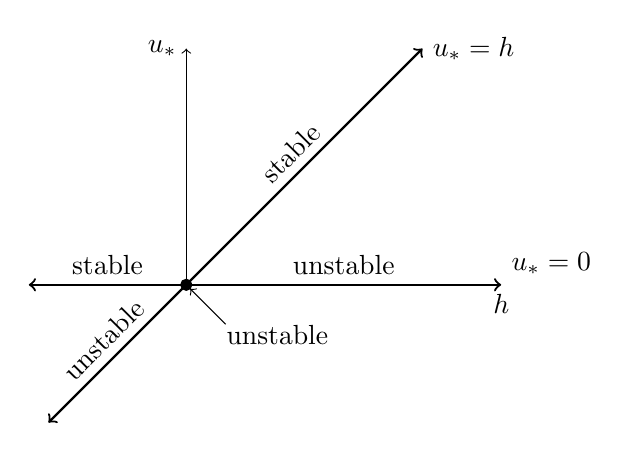
\begin{tikzpicture}
    %% axes
    \draw[<-] (0,3) node [left] {$u_*$} -- (0,0) -- (4,0) node [below] {$h$};
    %% lines
    \draw[thick,<-] (-2,0) -- (0,0)
    node[midway,above]{stable};
    \draw[thick,->] (0,0) -- (4,0)
    node[midway,above]{unstable}
    node[above right]{$u_*=0$};
    \draw[thick,<-] (-1.75,-1.75) -- (0,0)
    node[midway,above,sloped]{unstable};
    \draw[thick,->] (0,0) -- (3,3)
    node[midway,above,sloped]{stable}
    node[right]{$u_*=h$};
    \draw[fill] (0,0) circle (2pt);
    \draw[<-] (0.05,-0.05) -- (0.5,-0.5) node[near end,below right]{unstable};
  \end{tikzpicture}
  \caption{Bifurcation diagram for \#8a}
  \label{fig:8-bifurcation-diagram}
\end{figure}

\subsection{9}
\subsubsection*{Problem}
The following model contains fixed positive constants $a$, $b$ and a variable paramter $\lambda$.
\begin{equation*}
  u'=(\lambda - b) u-au^3
\end{equation*}

\begin{enumerate}
\item If $\lambda < b$  show that there is a single equilibrium and that it is
  asymptotically stable.
\item If $\lambda > b$ find all equilibria and determine their stability
\item Sketch the bifurcation diagram showing how equilibria vary with $\lambda$.
  Label each branch of the curves shown in the bifurcation diagram as stable or
  unstable.
\end{enumerate}

\subsubsection*{Solution}
Let $c=\lambda-b$, $f(u)=u'$ and define
\begin{equation}
  \label{eq:9-fu}
  \begin{aligned}
    f(u) = 0 \;\longrightarrow\;\;& cu-au^3=0 \\
    & u(c-au^2), \\
  \end{aligned}
\end{equation}
\begin{equation}
  \label{eq:9-d-fu}
  f'(u) = c-3au^2.
\end{equation}
The solutions to \cref{eq:9-fu} are $u_*=0,\,\pm\sqrt{c/a}$.
\begin{enumerate}
\item If $\lambda<b$, then $c<0$. Therefore the $\pm\sqrt{c/a}$ solutions are
  not real, so the only equilibrium is $u_*=0$. We will use \cref{eq:9-d-fu} and
  the derivative method to determine stability.
  \begin{equation*}
    \begin{aligned}
      f'(0) &= c.
    \end{aligned}
  \end{equation*}
  Since $c<0$, $u_*=0$ is stable.
\item If $\lambda>b$, then $c>0$. All solution are real in this case. We will use
  \cref{eq:9-d-fu} and the derivative method to determine stability.
  \begin{equation*}
    \begin{aligned}
      f'(0) &= c, \\
      f'(\pm\sqrt{c/a}) &= c-3\cancel{a}\frac{c}{\cancel{a}} \\
      &= -2c.
    \end{aligned}
  \end{equation*}
  Since $c>0$, $u_*=0$ is unstable and $u_*=\pm\sqrt{c/a}$ are stable.
\item Reference the bifurcation diagram in \cref{fig:9-bifurcation-diagram}.
\end{enumerate}

\begin{figure}
  \centering
  \begin{tikzpicture}[domain=2:4,label/.style={
      postaction={decorate,transform shape,
        decoration={markings, mark=at position .5 with \node #1;}}},
    x=2cm,y=1cm]
    \draw[<-] (0,3) node [left] {$u_*$} -- (0,0) -- (4,0) node [below] {$\lambda$};

    \draw[->,thick,label={[above]{stable}}] plot(\x,{sqrt(\x)})
    node[above right]{$u_*=\sqrt{\frac{\lambda-b}{a}}$};
    \draw[->,thick,label={[above]{stable}}] plot(\x,{-sqrt(\x)})
    node[above right]{$u_*=-\sqrt{\frac{\lambda-b}{a}}$};
    \draw[<-|,thick] (-1,0) -- (2,0) node[above left, very near end]{stable};
    \draw[->,thick] (2,0) -- (4,0)
    node[above right, at start]{unstable}
    node[above right]{$u_*=0$};
    \draw[dashed] (2,3) -- (2,-2.2) node[below left, very near end]{$b$};
  \end{tikzpicture}
  \caption{Bifurcation diagram for \#9}
  \label{fig:9-bifurcation-diagram}
\end{figure}

\subsection{13}
\subsubsection*{Problem}
A one-dimensional system is governed by the dynamical equation
\begin{equation}
  \label{eq:13-problem}
  u'=4u(a-u)-he^{-u}
\end{equation}
where $a$ and $h$ are positive constants. Draw a bifurcation diagram with
respect to the parameter $a$ while holding $h$ constant. Indicate the stable and
unstable branches.

\subsubsection*{Solution}
Reference \cref{fig:13-bifurcation-diagram}.
\begin{figure}
  \centering
  \begin{tikzpicture}[domain={-1+2*ln(2)}:4,label/.style={
      postaction={decorate,transform shape,
        decoration={markings, mark=at position .5 with \node #1;}}},
    x=2cm,y=1.5cm]
    \draw[<-] (0,3.25) node [left] {$u_*$} -- (0,0) -- (4,0) node [below] {$a$};

    \draw[->,thick,label={[below]{stable}}] plot({\x},{exp(-(\x-1)/2)});
    \draw[->,thick,label={[above]{unstable}}] plot({\x},{e-exp(-(\x-1)/2)});
    \draw[dashed] (0,{e}) -- (4,{e});
    \draw[fill] ({-1+2*ln(2)},{e/2}) circle (2pt) +(0.25,0) node[right]{unstable};
  \end{tikzpicture}
  \caption{Bifurcation diagram for \#13}
  \label{fig:13-bifurcation-diagram}
\end{figure}

\skiptooddpage{}
\section{Programming Minilab}
A simple model for the population of plants in a plant-herbivore ecosystem is
\begin{equation}
  \label{eq:minilab-problem}
  \od{p}{t} = rp\left( 1-\frac{p}{k} \right) - \frac{apq}{1+bp}, \quad p(0)=p_0
\end{equation}
Here $p(t)$ is the number of plants, $q$ is the constant number of herbivores,
$r$ and $k$ are constants that describe the growth rate of the plants, and $a$
and $b$ are constants that describe the consumption rate of the plants by the
herbivores. Here we perform a qualitative analysis to understand the behavior of
solutions of the model in \cref{eq:minilab-problem}. To quantify the population
sizes we introduce the dimensions $[p] = \text{Plant}$, $[q] =
\text{Herbivore}$, and $[t] = \text{Time}$. All constants are assumed positive.

\subsubsection*{Problem}
\begin{enumerate}
\item Find the dimensions of $r$, $k$, $a$, and $b$. Using the scales $t_c =
  1/r$ and $p_c = k$, show that the dimensionless version of
  \cref{eq:minilab-problem} takes the form
  \begin{equation}
    \label{eq:minilab-problem-a}
    \od{u}{\tau}=u(1-u)-\frac{hu}{1+cu},\quad u(0)=u_0
  \end{equation}
  where $u=p/p_c$, $\tau=t/t_c$, and $h,c$ are constants which you should
  identify.
\item Assuming $c>1$ is fixed, find (or characterize) all equilibrium solutions
  of \cref{eq:minilab-problem-a} and determine their stability in terms of the
  parameter $h>0$. Illustrate the results on a bifurcation diagram.
  \label{item:minilab-part-b}
\item Use \verb|program3.m| and \verb|plant.m| to numerically simulate the model
  in \cref{eq:minilab-problem-a}. Produce portraits of solutions for various
  $u_0$ when $c=4$ and a few different values of $h$. Do the simulations agree
  with the analysis in \cref{item:minilab-part-b}? According to the stability
  results in the bifurcation diagram, do solutions grow, decay, or remain
  constant?
\item For what range of the parameter $h$ would the plant population survive if
  $\tau\rightarrow\infty$, $c=4$, and $u(0)=1/4$? For what range of $h$, if any,
  would the plant population die out as $\tau\rightarrow\infty$?
\end{enumerate}
\subsubsection*{Solution}
\begin{enumerate}
\item Substituting the dimensions of each variable for the first expression on
  the right side of \cref{eq:minilab-problem} yields
  \begin{equation}
    \label{eq:minilab-rhs-1}
    \begin{aligned}
      PT^{-1} &= rp(1-\frac{p}{k}) \\
      &= rP - \frac{rP^2}{k}.
    \end{aligned}
  \end{equation}
  Both of the expressions on the right side of \cref{eq:minilab-rhs-1} must have
  the same dimensions. Thus
  $$\implies r=T^{-1}.$$ and
  \begin{equation*}
    \begin{aligned}
      PT^{-1} &= \frac{rP^2}{k} \\
      &= \frac{P^2T^{-1}}{k} \\
      \implies k&= P. \\
    \end{aligned}
  \end{equation*}

  Substituting the dimensions of each variable for the second expression on the
  right side of \cref{eq:minilab-problem} yields
  \begin{equation}
    \label{eq:minilab-rhs-2}
    \begin{aligned}
      PT^{-1} &= \frac{apq}{1+bp} \\
      &= \frac{HPa}{1+Pb} \\
      PT^{-1}+P^2T^{-1}b &= HPa \\
      PT^{-1} &= HPa - P^2T^{-1}b \\
    \end{aligned}
  \end{equation}

  Each expression on the right side of \cref{eq:minilab-rhs-2} must have the
  same dimensions. Thus
  \begin{equation*}
    \begin{aligned}
      \implies a&=H^{-1}T^{-1} \quad\text{and} \\
      \implies b&=P^{-1}. \\
    \end{aligned}
  \end{equation*}

  Now we may obtain the dimensionless form of \cref{eq:minilab-problem}.
  \begin{equation}
    \begin{aligned}
      \od{u}{\tau} &= \frac{t_c}{p_c}\od{p}{t} \\
      &= \frac{1}{rk}\left(rp(1-\frac{p}{k})\right)-\frac{apq}{1+bp} \\
      &= \frac{1}{rk}\left(ruk\left(1-\frac{u\cancel{k}}{\cancel{k}}\right)\right) - \frac{aukq}{1+bk} \\
      &= \cancel{\frac{1}{rk}}(\cancel{r}u\cancel{k}-\cancel{r}u^2\cancel{k})- \frac{aukq}{1+bk} \\
      &= u-u^2 - \frac{aukq}{1+bk} \\
      &= u(1-u) - \frac{(akq)u}{1+(bk)u}
    \end{aligned}
  \end{equation}
  From this we may conclude
  \begin{equation*}
    \begin{aligned}
      \implies h&=akq \\
      \implies c&=bk. \\
    \end{aligned}
  \end{equation*}
  This agrees with \cref{eq:minilab-problem-a}.
\item Reference \cref{fig:minilab-bifurcation-diagram}. The solutions seem to
  generally decay as $h$ grows.
  \begin{figure}
    \centering
    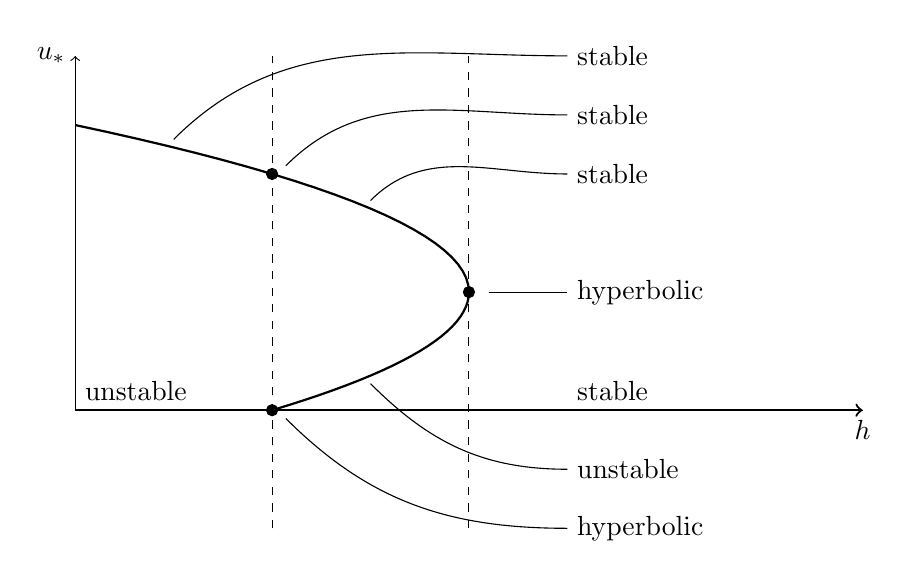
\begin{tikzpicture}[domain=0:{sqrt(2)},label/.style={
        postaction={decorate,transform shape,
          decoration={markings, mark=at position .5 with \node #1;}}},x=2.5cm,y=1.5cm]
      \draw[<-] (0,3) node [left] {$u_*$} -- (0,0) -- (4,0) node [below] {$h$};

      \draw[-,thick] plot(-\x^2+2,{\x+1});
      \draw[-,thick,domain=0:1] plot(-\x^2+2,{-\x+1});
      \draw[->,thick] (0,0) -- (4,0);
      \draw (2.5,0) node[above right]{stable};

      \draw[dashed] (1,-1) -- (1,3);
      \draw[dashed] (2,-1) -- (2,3);

      \draw[fill] (1,2) circle (2pt);
      \draw[fill] (1,0) circle (2pt);
      \draw[fill] (2,1) circle (2pt);

      \draw[-] (1.5,{sqrt(1.5)-1}) to [out=-45,in=180] (2.5,-0.5)
      node[right]{unstable};
      \draw[-] (1.5,{-sqrt(1.5)+3}) to [out=45,in=180] (2.5,2)
      node[right]{stable};

      \draw[-] (1+0.07,{sqrt(1)-1-0.07}) to [out=-45,in=180] (2.5,-1)
      node[right]{hyperbolic};
      \draw[-] (1+0.07,{-sqrt(1)+3+0.07}) to [out=45,in=180] (2.5,2.5)
      node[right]{stable};

      \draw[-] (0.5,{-sqrt(0.5)+3}) to [out=45,in=180] (2.5,3)
      node[right]{stable};

      \draw[-] (2+0.1,1) -- (2.5,1) node[right]{hyperbolic};

      \draw (0,0) node[above right]{unstable};
    \end{tikzpicture}
    \caption{Bifurcation diagram for minilab}
    \label{fig:minilab-bifurcation-diagram}
  \end{figure}
\item Reference \cref{fig:minilab-solution-curves}. The solutions agree with the
  analysis.

  \begin{figure}
    \begin{subfigure}[b]{0.45\textwidth}
      \resizebox{\linewidth}{!}{
        \begin{tikzpicture}
          \centering
          \begin{axis}[domain=0:50, view={0}{90}, xlabel=$\tau$, ylabel=$u$]
            \foreach \i in {1,...,50} {
              \addplot3[very thin] table {src-bin/minilab-1-\i.mat};
            }
          \end{axis}
        \end{tikzpicture}}
      \caption{$h=0.8$}
    \end{subfigure}
    \begin{subfigure}[b]{0.45\textwidth}
      \resizebox{\linewidth}{!}{
        \begin{tikzpicture}
          \centering
          \begin{axis}[domain=0:50, view={0}{90}, xlabel=$\tau$, ylabel=$u$]
            \foreach \i in {1,...,50} {
              \addplot3[very thin] table {src-bin/minilab-2-\i.mat};
            }
          \end{axis}
        \end{tikzpicture}}
      \caption{$h=1.0$}
    \end{subfigure}
    \begin{subfigure}[b]{0.45\textwidth}
      \resizebox{\linewidth}{!}{
        \begin{tikzpicture}
          \centering
          \begin{axis}[domain=0:50, view={0}{90}, xlabel=$\tau$, ylabel=$u$]
            \foreach \i in {1,...,50} {
              \addplot3[very thin] table {src-bin/minilab-3-\i.mat};
            }
          \end{axis}
        \end{tikzpicture}}
      \caption{$h=1.5$}
    \end{subfigure}
    \begin{subfigure}[b]{0.45\textwidth}
      \resizebox{\linewidth}{!}{
        \begin{tikzpicture}
          \centering
          \begin{axis}[domain=0:50, view={0}{90}, xlabel=$\tau$, ylabel=$u$]
            \foreach \i in {1,...,50} {
              \addplot3[very thin] table {src-bin/minilab-4-\i.mat};
            }
          \end{axis}
        \end{tikzpicture}}
      \caption{$h=1.6$}
    \end{subfigure}
    \begin{subfigure}[b]{0.45\textwidth}
      \resizebox{\linewidth}{!}{
        \begin{tikzpicture}
          \centering
          \begin{axis}[domain=0:50, view={0}{90}, xlabel=$\tau$, ylabel=$u$]
            \foreach \i in {1,...,50} {
              \addplot3[very thin] table {src-bin/minilab-5-\i.mat};
            }
          \end{axis}
        \end{tikzpicture}}
      \caption{$h=2.0$}
    \end{subfigure}
    \caption{Solution curves for various $h$}
    \label{fig:minilab-solution-curves}
  \end{figure}
\item The plant population will survive when $0<h\le1.5$. The plant population
  will die out when $h>1.5$.
\end{enumerate}
\end{document}




% \begin{subfigure}{0.45\textwidth}
%   \hspace{-4em}
%   \scalebox{0.45}{% Title: glps_renderer figure
% Creator: GL2PS 1.3.9, (C) 1999-2015 C. Geuzaine
% For: Octave
% CreationDate: Mon Feb 15 07:59:24 2016
\setlength{\unitlength}{1pt}
\begin{picture}(0,0)
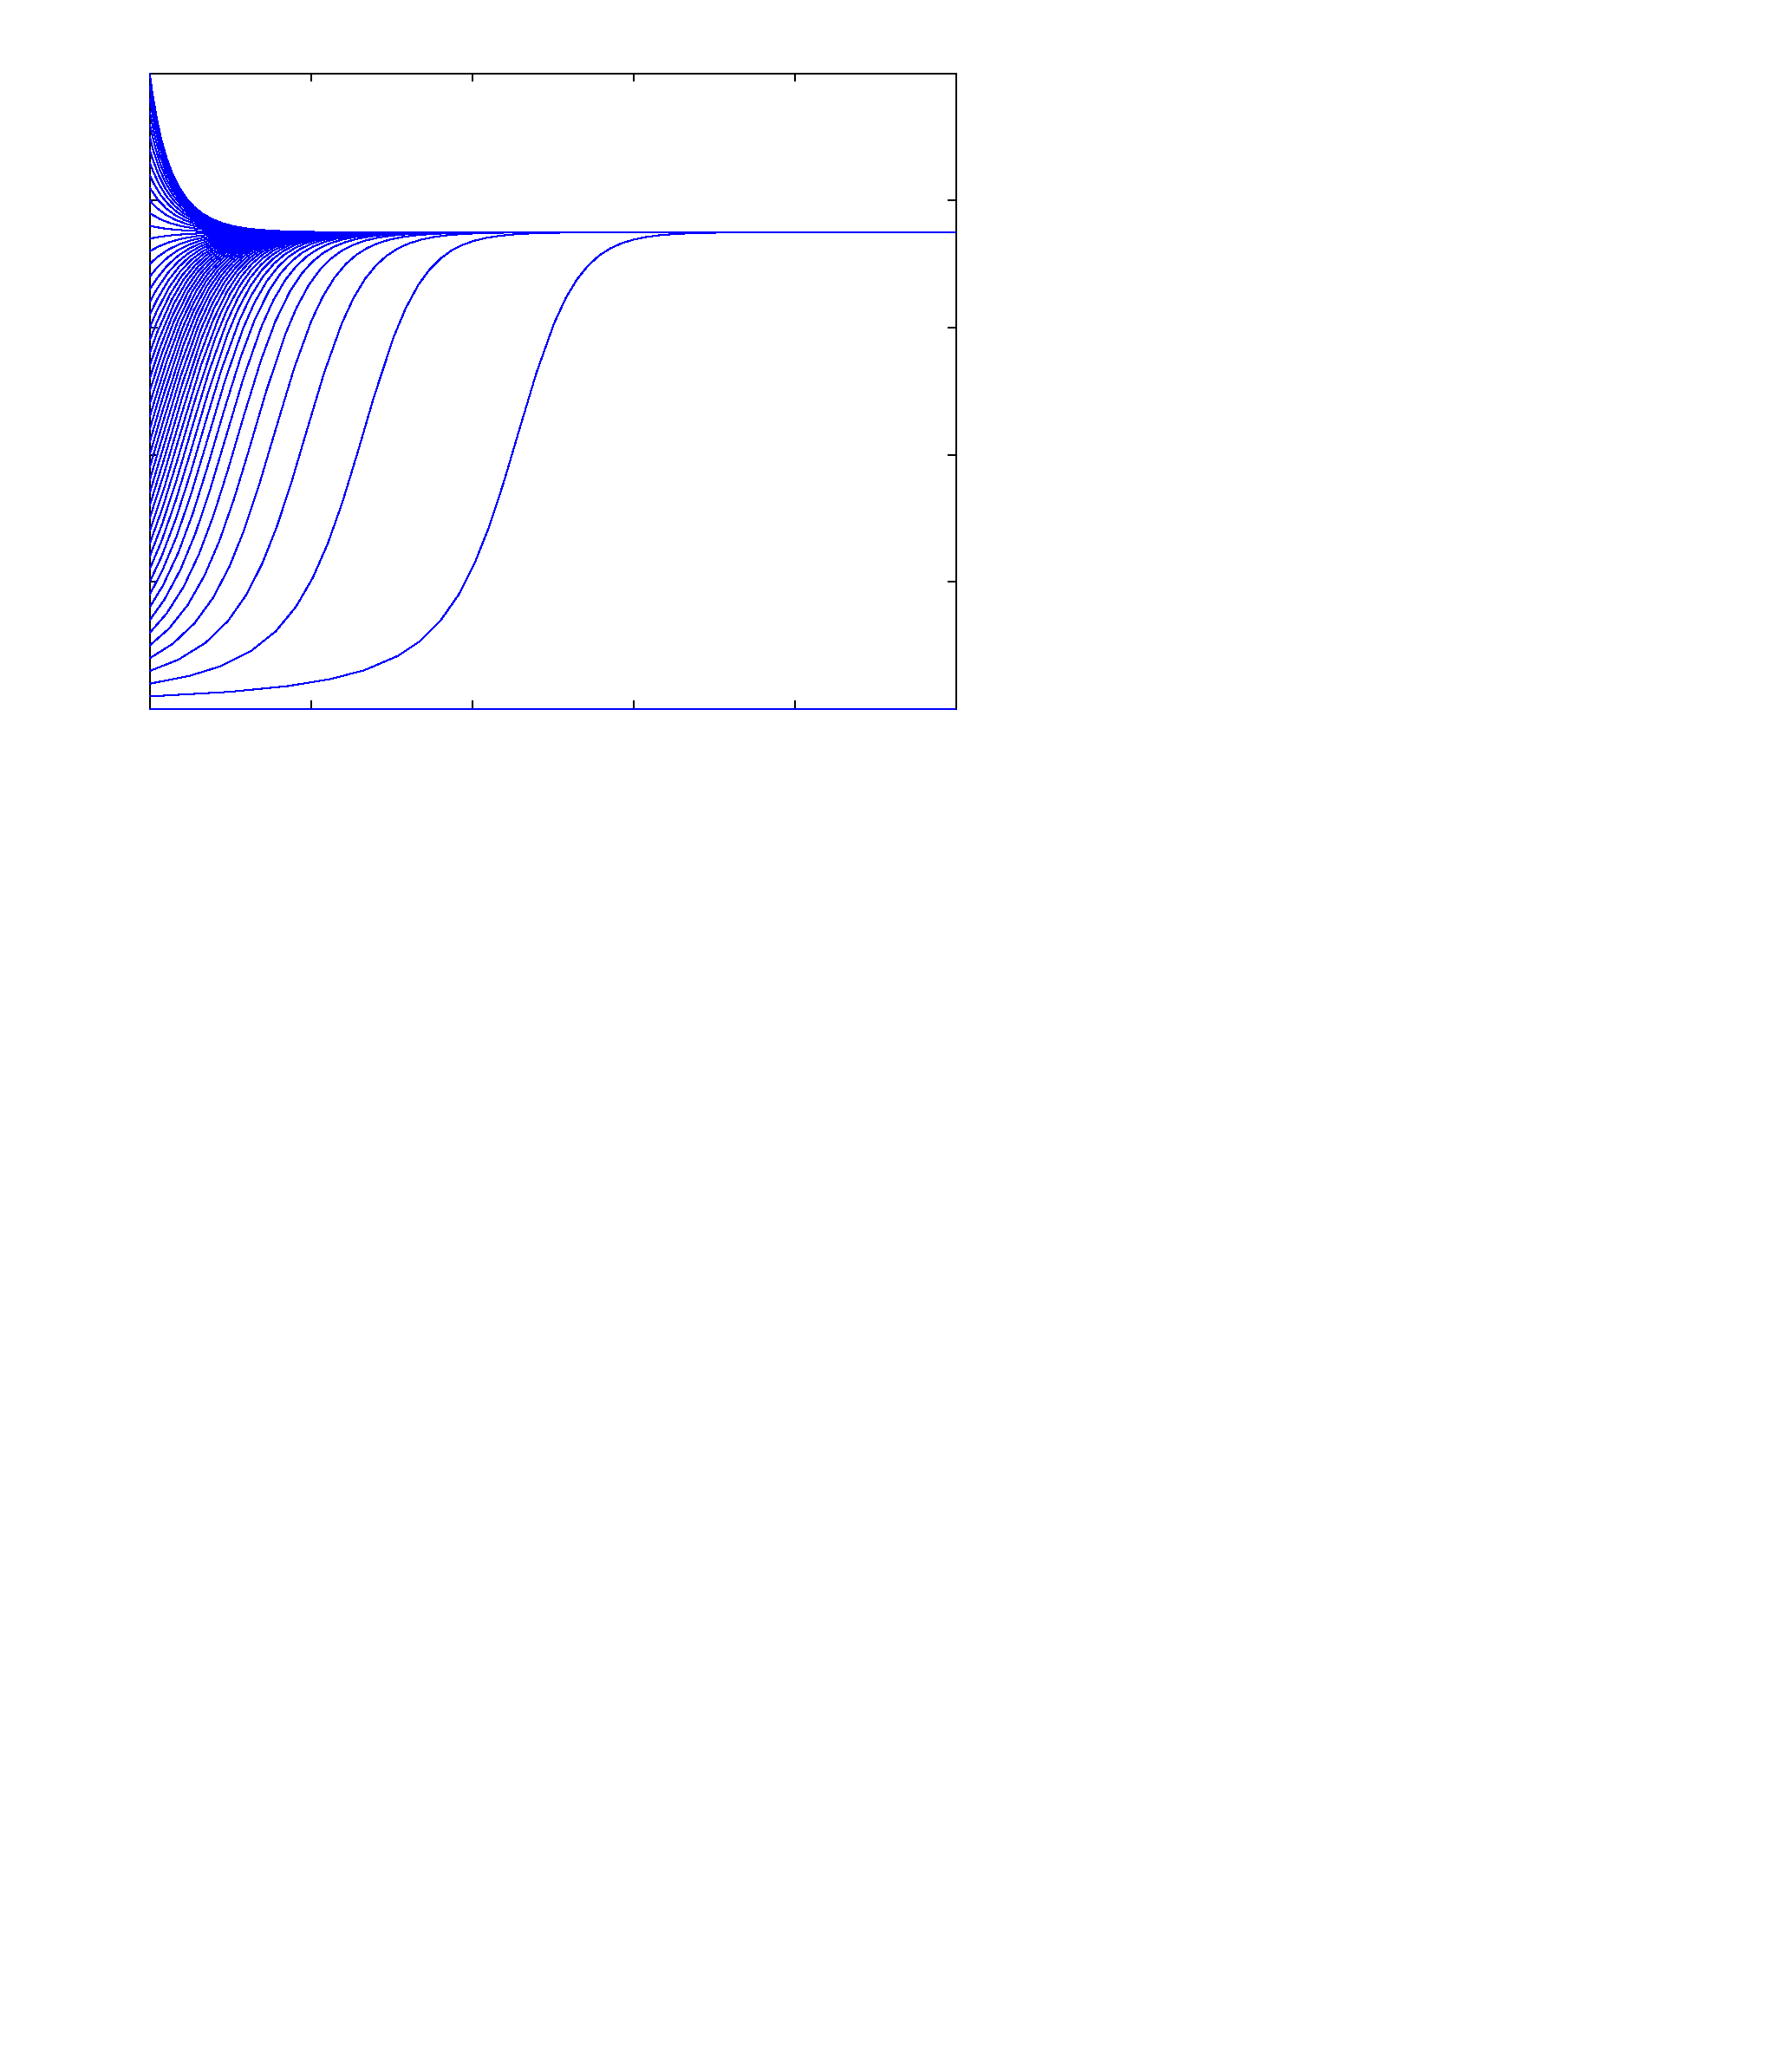
\includegraphics{prog3_fig2-inc}
\end{picture}%
\begin{picture}(976,1119)(0,0)
\fontsize{10}{0}
\selectfont\put(74.88,729.519){\makebox(0,0)[t]{\textcolor[rgb]{0,0,0}{{0}}}}
\fontsize{10}{0}
\selectfont\put(164.16,729.519){\makebox(0,0)[t]{\textcolor[rgb]{0,0,0}{{10}}}}
\fontsize{10}{0}
\selectfont\put(253.44,729.519){\makebox(0,0)[t]{\textcolor[rgb]{0,0,0}{{20}}}}
\fontsize{10}{0}
\selectfont\put(342.72,729.519){\makebox(0,0)[t]{\textcolor[rgb]{0,0,0}{{30}}}}
\fontsize{10}{0}
\selectfont\put(432,729.519){\makebox(0,0)[t]{\textcolor[rgb]{0,0,0}{{40}}}}
\fontsize{10}{0}
\selectfont\put(521.28,729.519){\makebox(0,0)[t]{\textcolor[rgb]{0,0,0}{{50}}}}
\fontsize{10}{0}
\selectfont\put(69.8755,734.52){\makebox(0,0)[r]{\textcolor[rgb]{0,0,0}{{0}}}}
\fontsize{10}{0}
\selectfont\put(69.8755,804.936){\makebox(0,0)[r]{\textcolor[rgb]{0,0,0}{{0.2}}}}
\fontsize{10}{0}
\selectfont\put(69.8755,875.352){\makebox(0,0)[r]{\textcolor[rgb]{0,0,0}{{0.4}}}}
\fontsize{10}{0}
\selectfont\put(69.8755,945.768){\makebox(0,0)[r]{\textcolor[rgb]{0,0,0}{{0.6}}}}
\fontsize{10}{0}
\selectfont\put(69.8755,1016.18){\makebox(0,0)[r]{\textcolor[rgb]{0,0,0}{{0.8}}}}
\fontsize{10}{0}
\selectfont\put(69.8755,1086.6){\makebox(0,0)[r]{\textcolor[rgb]{0,0,0}{{1}}}}
\fontsize{10}{0}
\selectfont\put(298.08,718.519){\makebox(0,0)[t]{\textcolor[rgb]{0,0,0}{{$\tau$}}}}
\fontsize{10}{0}
\selectfont\put(50.8755,910.56){\rotatebox{90}{\makebox(0,0)[b]{\textcolor[rgb]{0,0,0}{{$u$}}}}}
\fontsize{10}{0}
\selectfont\put(298.08,1096.6){\makebox(0,0)[b]{\textcolor[rgb]{0,0,0}{{Solution curves for different initial conditions, $h=1.0$}}}}
\end{picture}
}
%   \vspace{-28.5em}
%   \caption{$h=1.0$}
% \end{subfigure}
% \begin{subfigure}{0.45\textwidth}
%   \hspace{-4em}
%   \scalebox{0.45}{% Title: glps_renderer figure
% Creator: GL2PS 1.3.9, (C) 1999-2015 C. Geuzaine
% For: Octave
% CreationDate: Mon Feb 15 08:00:28 2016
\setlength{\unitlength}{1pt}
\begin{picture}(0,0)
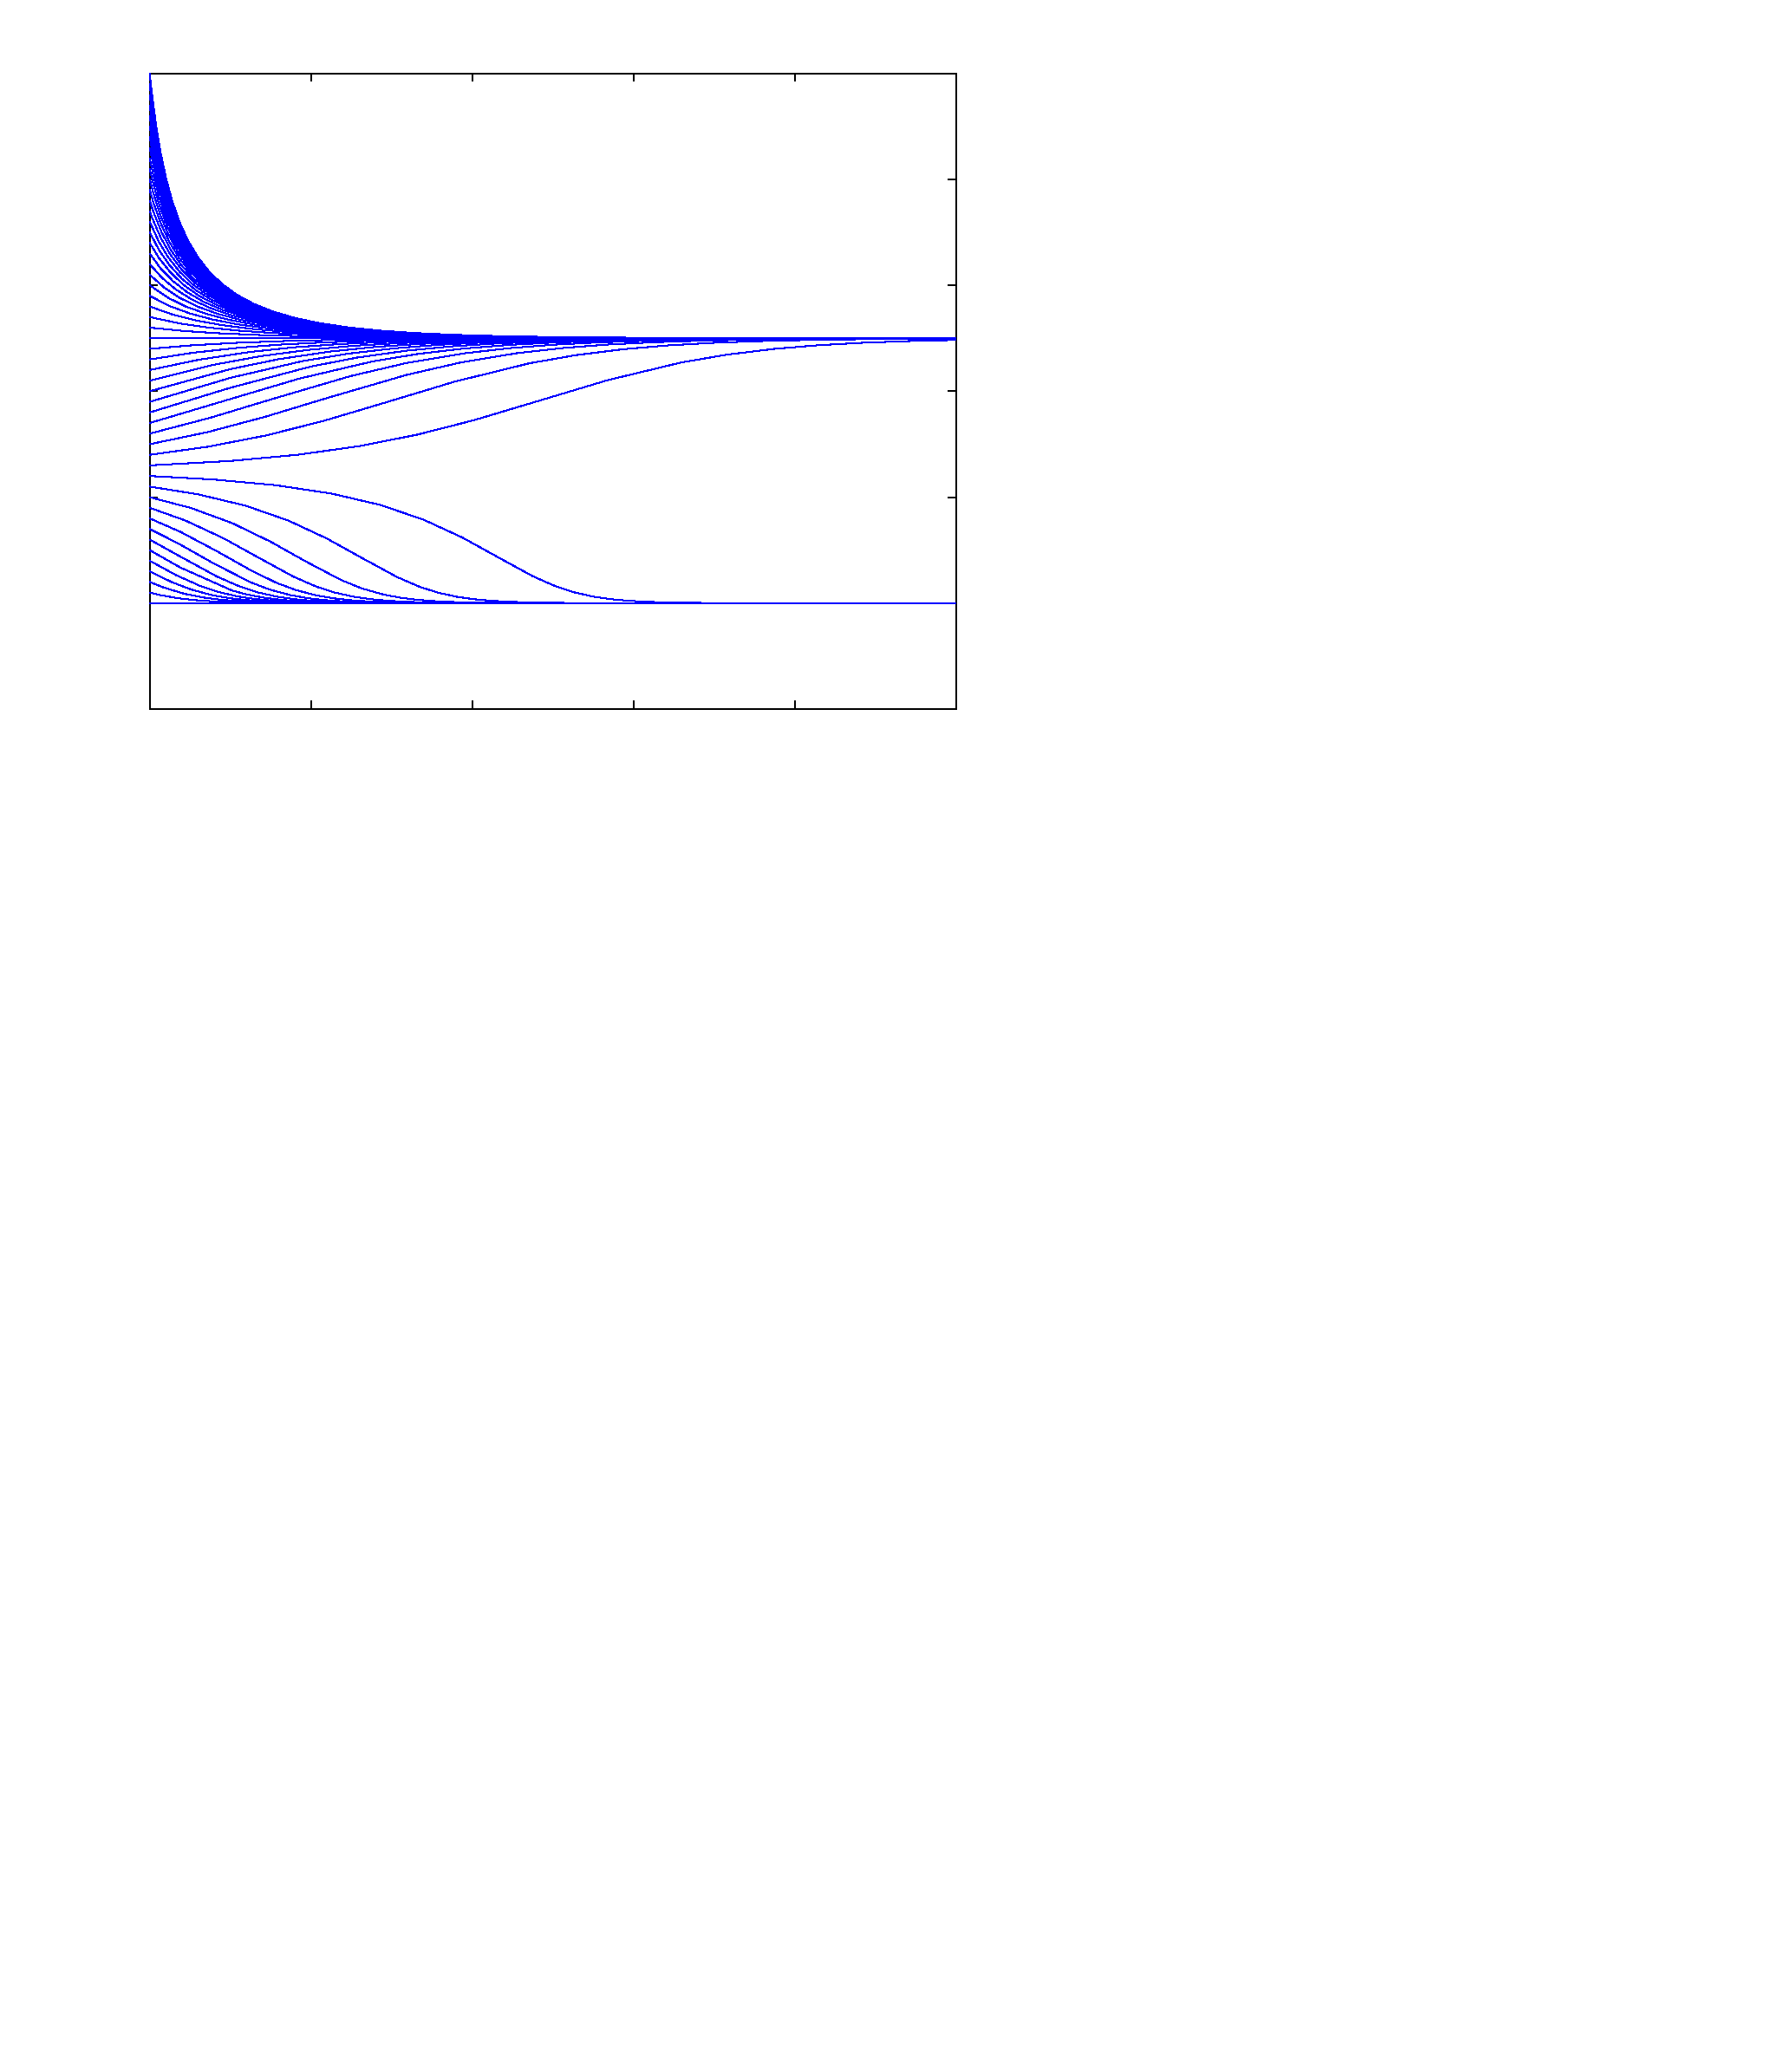
\includegraphics{prog3_fig3-inc}
\end{picture}%
\begin{picture}(976,1119)(0,0)
\fontsize{10}{0}
\selectfont\put(74.88,729.519){\makebox(0,0)[t]{\textcolor[rgb]{0,0,0}{{0}}}}
\fontsize{10}{0}
\selectfont\put(164.16,729.519){\makebox(0,0)[t]{\textcolor[rgb]{0,0,0}{{10}}}}
\fontsize{10}{0}
\selectfont\put(253.44,729.519){\makebox(0,0)[t]{\textcolor[rgb]{0,0,0}{{20}}}}
\fontsize{10}{0}
\selectfont\put(342.72,729.519){\makebox(0,0)[t]{\textcolor[rgb]{0,0,0}{{30}}}}
\fontsize{10}{0}
\selectfont\put(432,729.519){\makebox(0,0)[t]{\textcolor[rgb]{0,0,0}{{40}}}}
\fontsize{10}{0}
\selectfont\put(521.28,729.519){\makebox(0,0)[t]{\textcolor[rgb]{0,0,0}{{50}}}}
\fontsize{10}{0}
\selectfont\put(69.8755,734.52){\makebox(0,0)[r]{\textcolor[rgb]{0,0,0}{{-0.2}}}}
\fontsize{10}{0}
\selectfont\put(69.8755,793.2){\makebox(0,0)[r]{\textcolor[rgb]{0,0,0}{{0}}}}
\fontsize{10}{0}
\selectfont\put(69.8755,851.88){\makebox(0,0)[r]{\textcolor[rgb]{0,0,0}{{0.2}}}}
\fontsize{10}{0}
\selectfont\put(69.8755,910.56){\makebox(0,0)[r]{\textcolor[rgb]{0,0,0}{{0.4}}}}
\fontsize{10}{0}
\selectfont\put(69.8755,969.24){\makebox(0,0)[r]{\textcolor[rgb]{0,0,0}{{0.6}}}}
\fontsize{10}{0}
\selectfont\put(69.8755,1027.92){\makebox(0,0)[r]{\textcolor[rgb]{0,0,0}{{0.8}}}}
\fontsize{10}{0}
\selectfont\put(69.8755,1086.6){\makebox(0,0)[r]{\textcolor[rgb]{0,0,0}{{1}}}}
\fontsize{10}{0}
\selectfont\put(298.08,718.519){\makebox(0,0)[t]{\textcolor[rgb]{0,0,0}{{$\tau$}}}}
\fontsize{10}{0}
\selectfont\put(46.8755,910.56){\rotatebox{90}{\makebox(0,0)[b]{\textcolor[rgb]{0,0,0}{{$u$}}}}}
\fontsize{10}{0}
\selectfont\put(298.08,1096.6){\makebox(0,0)[b]{\textcolor[rgb]{0,0,0}{{Solution curves for different initial conditions, $h=1.5$}}}}
\end{picture}
}
%   \vspace{-28.5em}
%   \caption{$h=1.5$}
% \end{subfigure}
% \begin{subfigure}{0.45\textwidth}
%   \hspace{-4em}
%   \scalebox{0.45}{% Title: glps_renderer figure
% Creator: GL2PS 1.3.9, (C) 1999-2015 C. Geuzaine
% For: Octave
% CreationDate: Mon Feb 15 08:02:01 2016
\setlength{\unitlength}{1pt}
\begin{picture}(0,0)
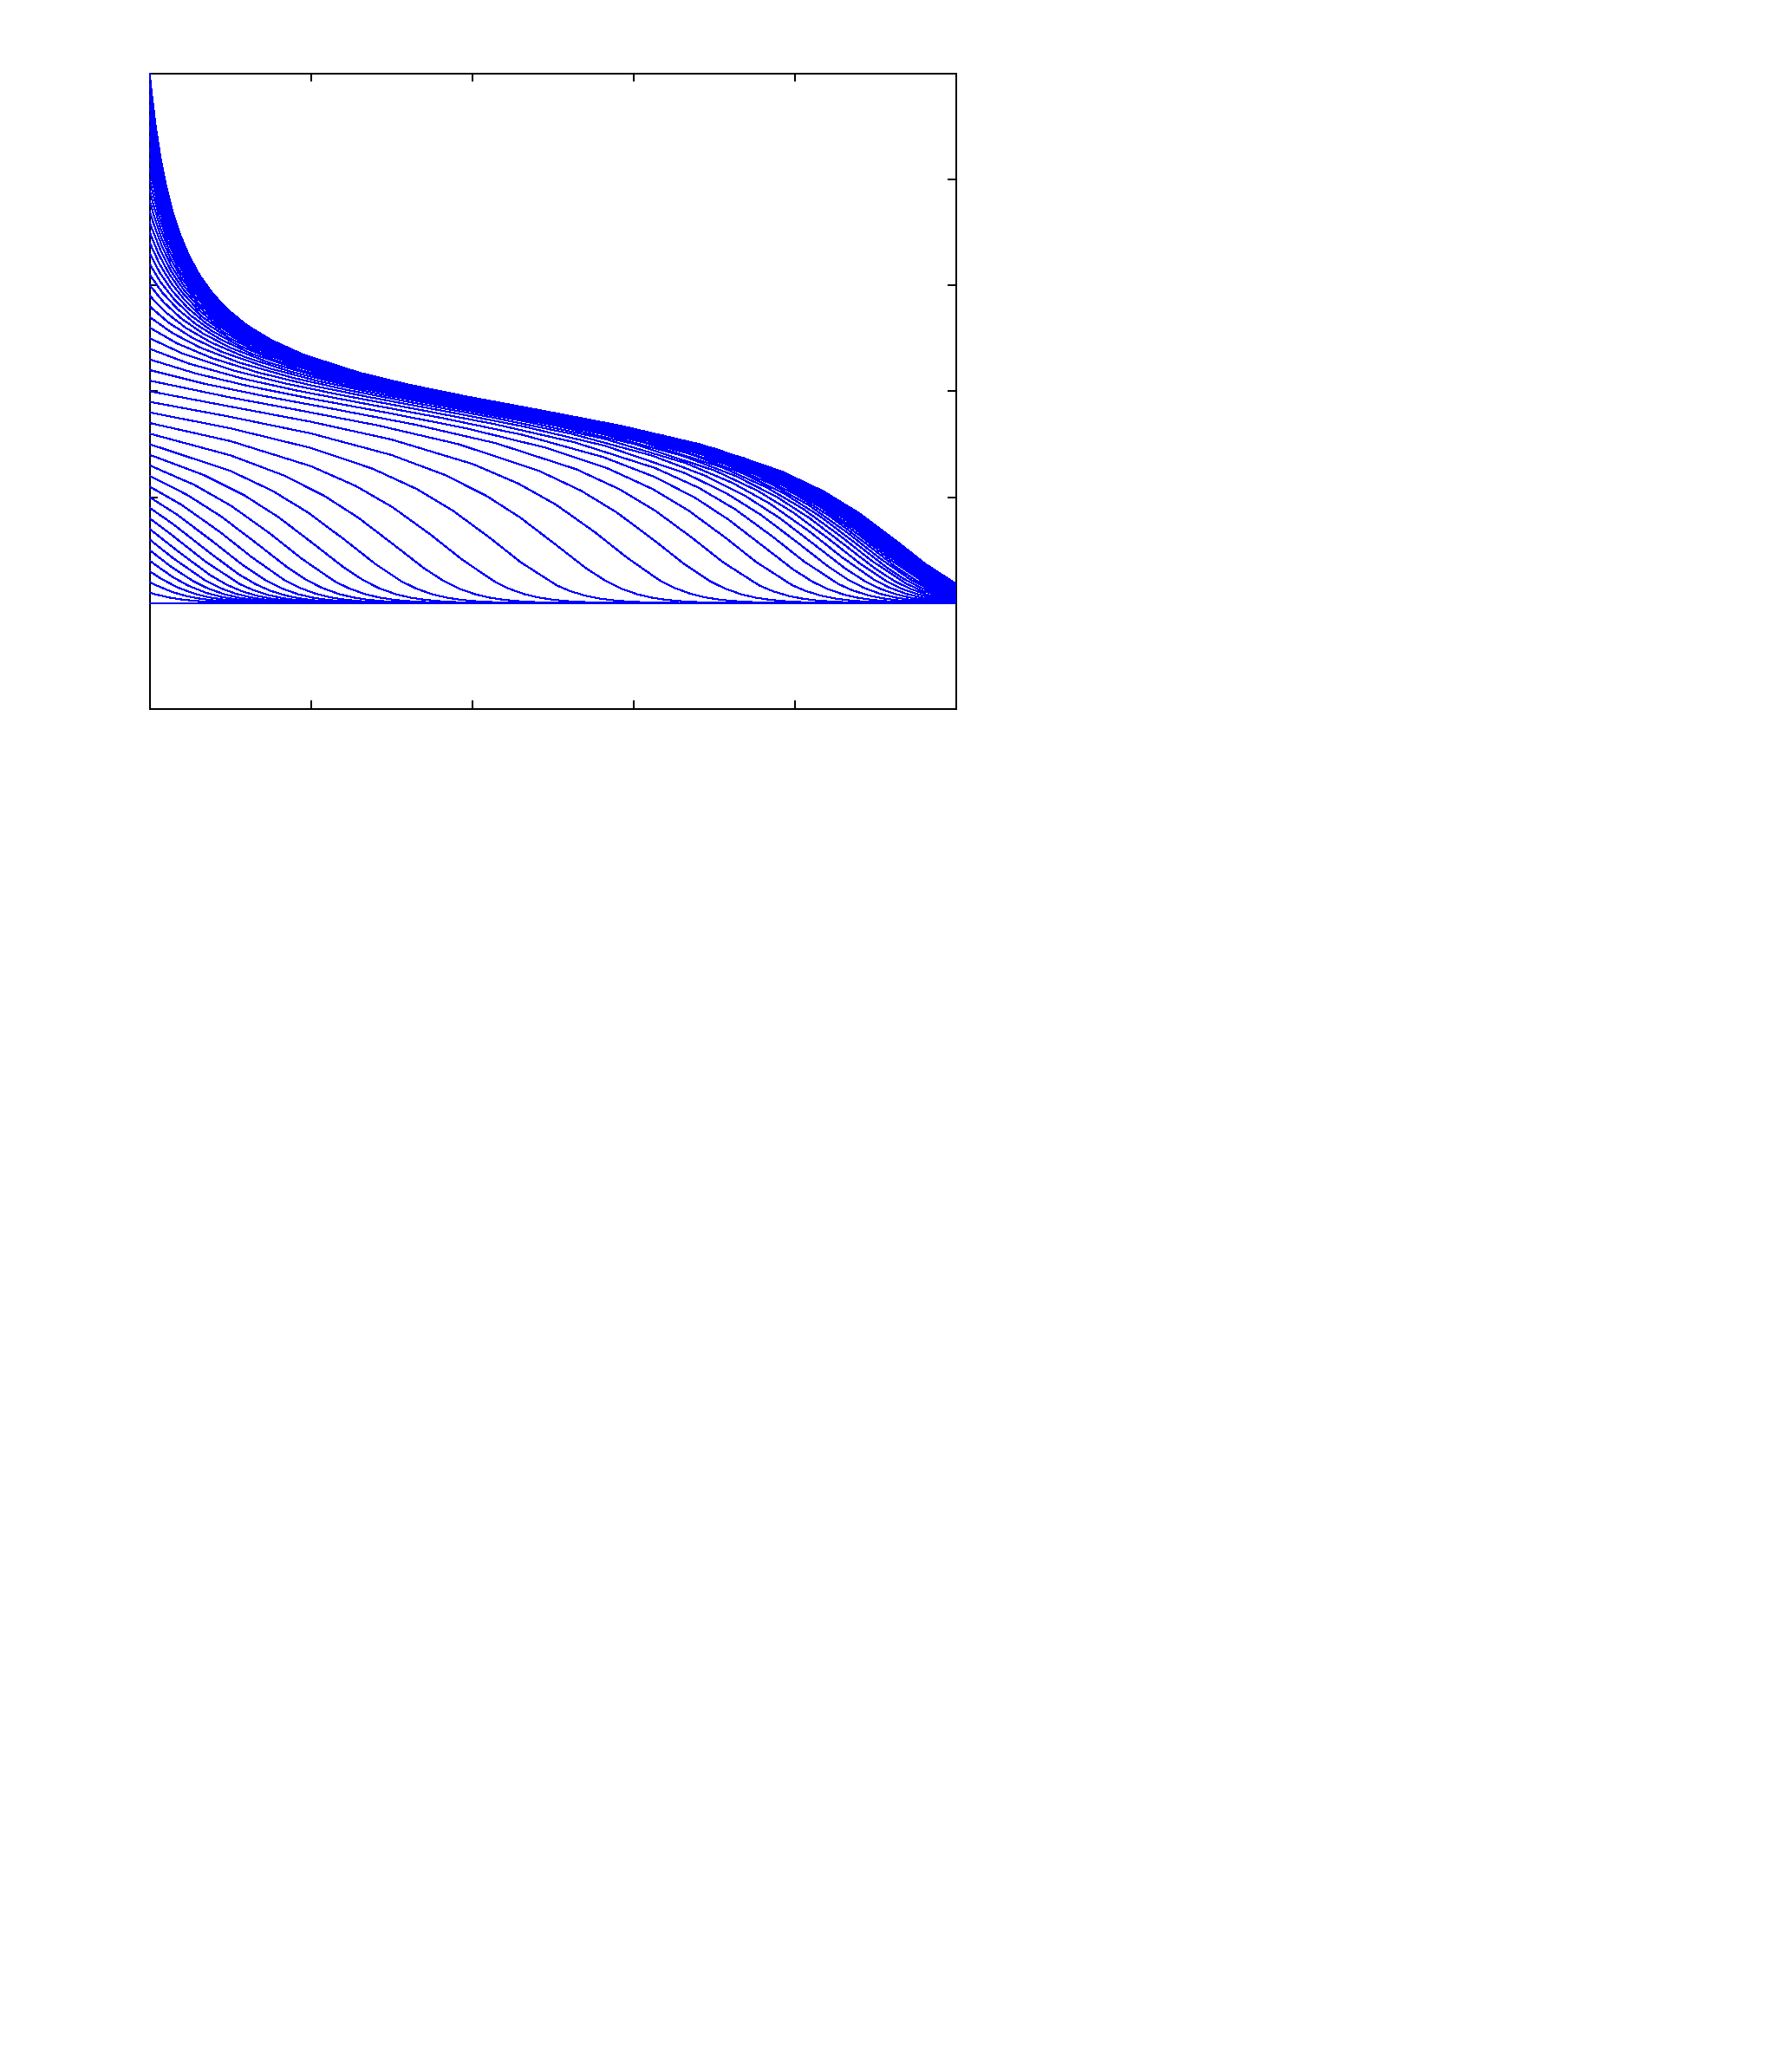
\includegraphics{prog3_fig4-inc}
\end{picture}%
\begin{picture}(976,1119)(0,0)
\fontsize{10}{0}
\selectfont\put(74.88,729.519){\makebox(0,0)[t]{\textcolor[rgb]{0,0,0}{{0}}}}
\fontsize{10}{0}
\selectfont\put(164.16,729.519){\makebox(0,0)[t]{\textcolor[rgb]{0,0,0}{{10}}}}
\fontsize{10}{0}
\selectfont\put(253.44,729.519){\makebox(0,0)[t]{\textcolor[rgb]{0,0,0}{{20}}}}
\fontsize{10}{0}
\selectfont\put(342.72,729.519){\makebox(0,0)[t]{\textcolor[rgb]{0,0,0}{{30}}}}
\fontsize{10}{0}
\selectfont\put(432,729.519){\makebox(0,0)[t]{\textcolor[rgb]{0,0,0}{{40}}}}
\fontsize{10}{0}
\selectfont\put(521.28,729.519){\makebox(0,0)[t]{\textcolor[rgb]{0,0,0}{{50}}}}
\fontsize{10}{0}
\selectfont\put(69.8755,734.52){\makebox(0,0)[r]{\textcolor[rgb]{0,0,0}{{-0.2}}}}
\fontsize{10}{0}
\selectfont\put(69.8755,793.2){\makebox(0,0)[r]{\textcolor[rgb]{0,0,0}{{0}}}}
\fontsize{10}{0}
\selectfont\put(69.8755,851.88){\makebox(0,0)[r]{\textcolor[rgb]{0,0,0}{{0.2}}}}
\fontsize{10}{0}
\selectfont\put(69.8755,910.56){\makebox(0,0)[r]{\textcolor[rgb]{0,0,0}{{0.4}}}}
\fontsize{10}{0}
\selectfont\put(69.8755,969.24){\makebox(0,0)[r]{\textcolor[rgb]{0,0,0}{{0.6}}}}
\fontsize{10}{0}
\selectfont\put(69.8755,1027.92){\makebox(0,0)[r]{\textcolor[rgb]{0,0,0}{{0.8}}}}
\fontsize{10}{0}
\selectfont\put(69.8755,1086.6){\makebox(0,0)[r]{\textcolor[rgb]{0,0,0}{{1}}}}
\fontsize{10}{0}
\selectfont\put(298.08,718.519){\makebox(0,0)[t]{\textcolor[rgb]{0,0,0}{{$\tau$}}}}
\fontsize{10}{0}
\selectfont\put(46.8755,910.56){\rotatebox{90}{\makebox(0,0)[b]{\textcolor[rgb]{0,0,0}{{$u$}}}}}
\fontsize{10}{0}
\selectfont\put(298.08,1096.6){\makebox(0,0)[b]{\textcolor[rgb]{0,0,0}{{Solution curves for different initial conditions, $h=1.6$}}}}
\end{picture}
}
%   \vspace{-28.5em}
%   \caption{$h=1.6$}
% \end{subfigure}~
% \begin{subfigure}{0.45\textwidth}
%   \hspace{-4em}
%   \scalebox{0.45}{% Title: glps_renderer figure
% Creator: GL2PS 1.3.9, (C) 1999-2015 C. Geuzaine
% For: Octave
% CreationDate: Mon Feb 15 08:02:21 2016
\setlength{\unitlength}{1pt}
\begin{picture}(0,0)
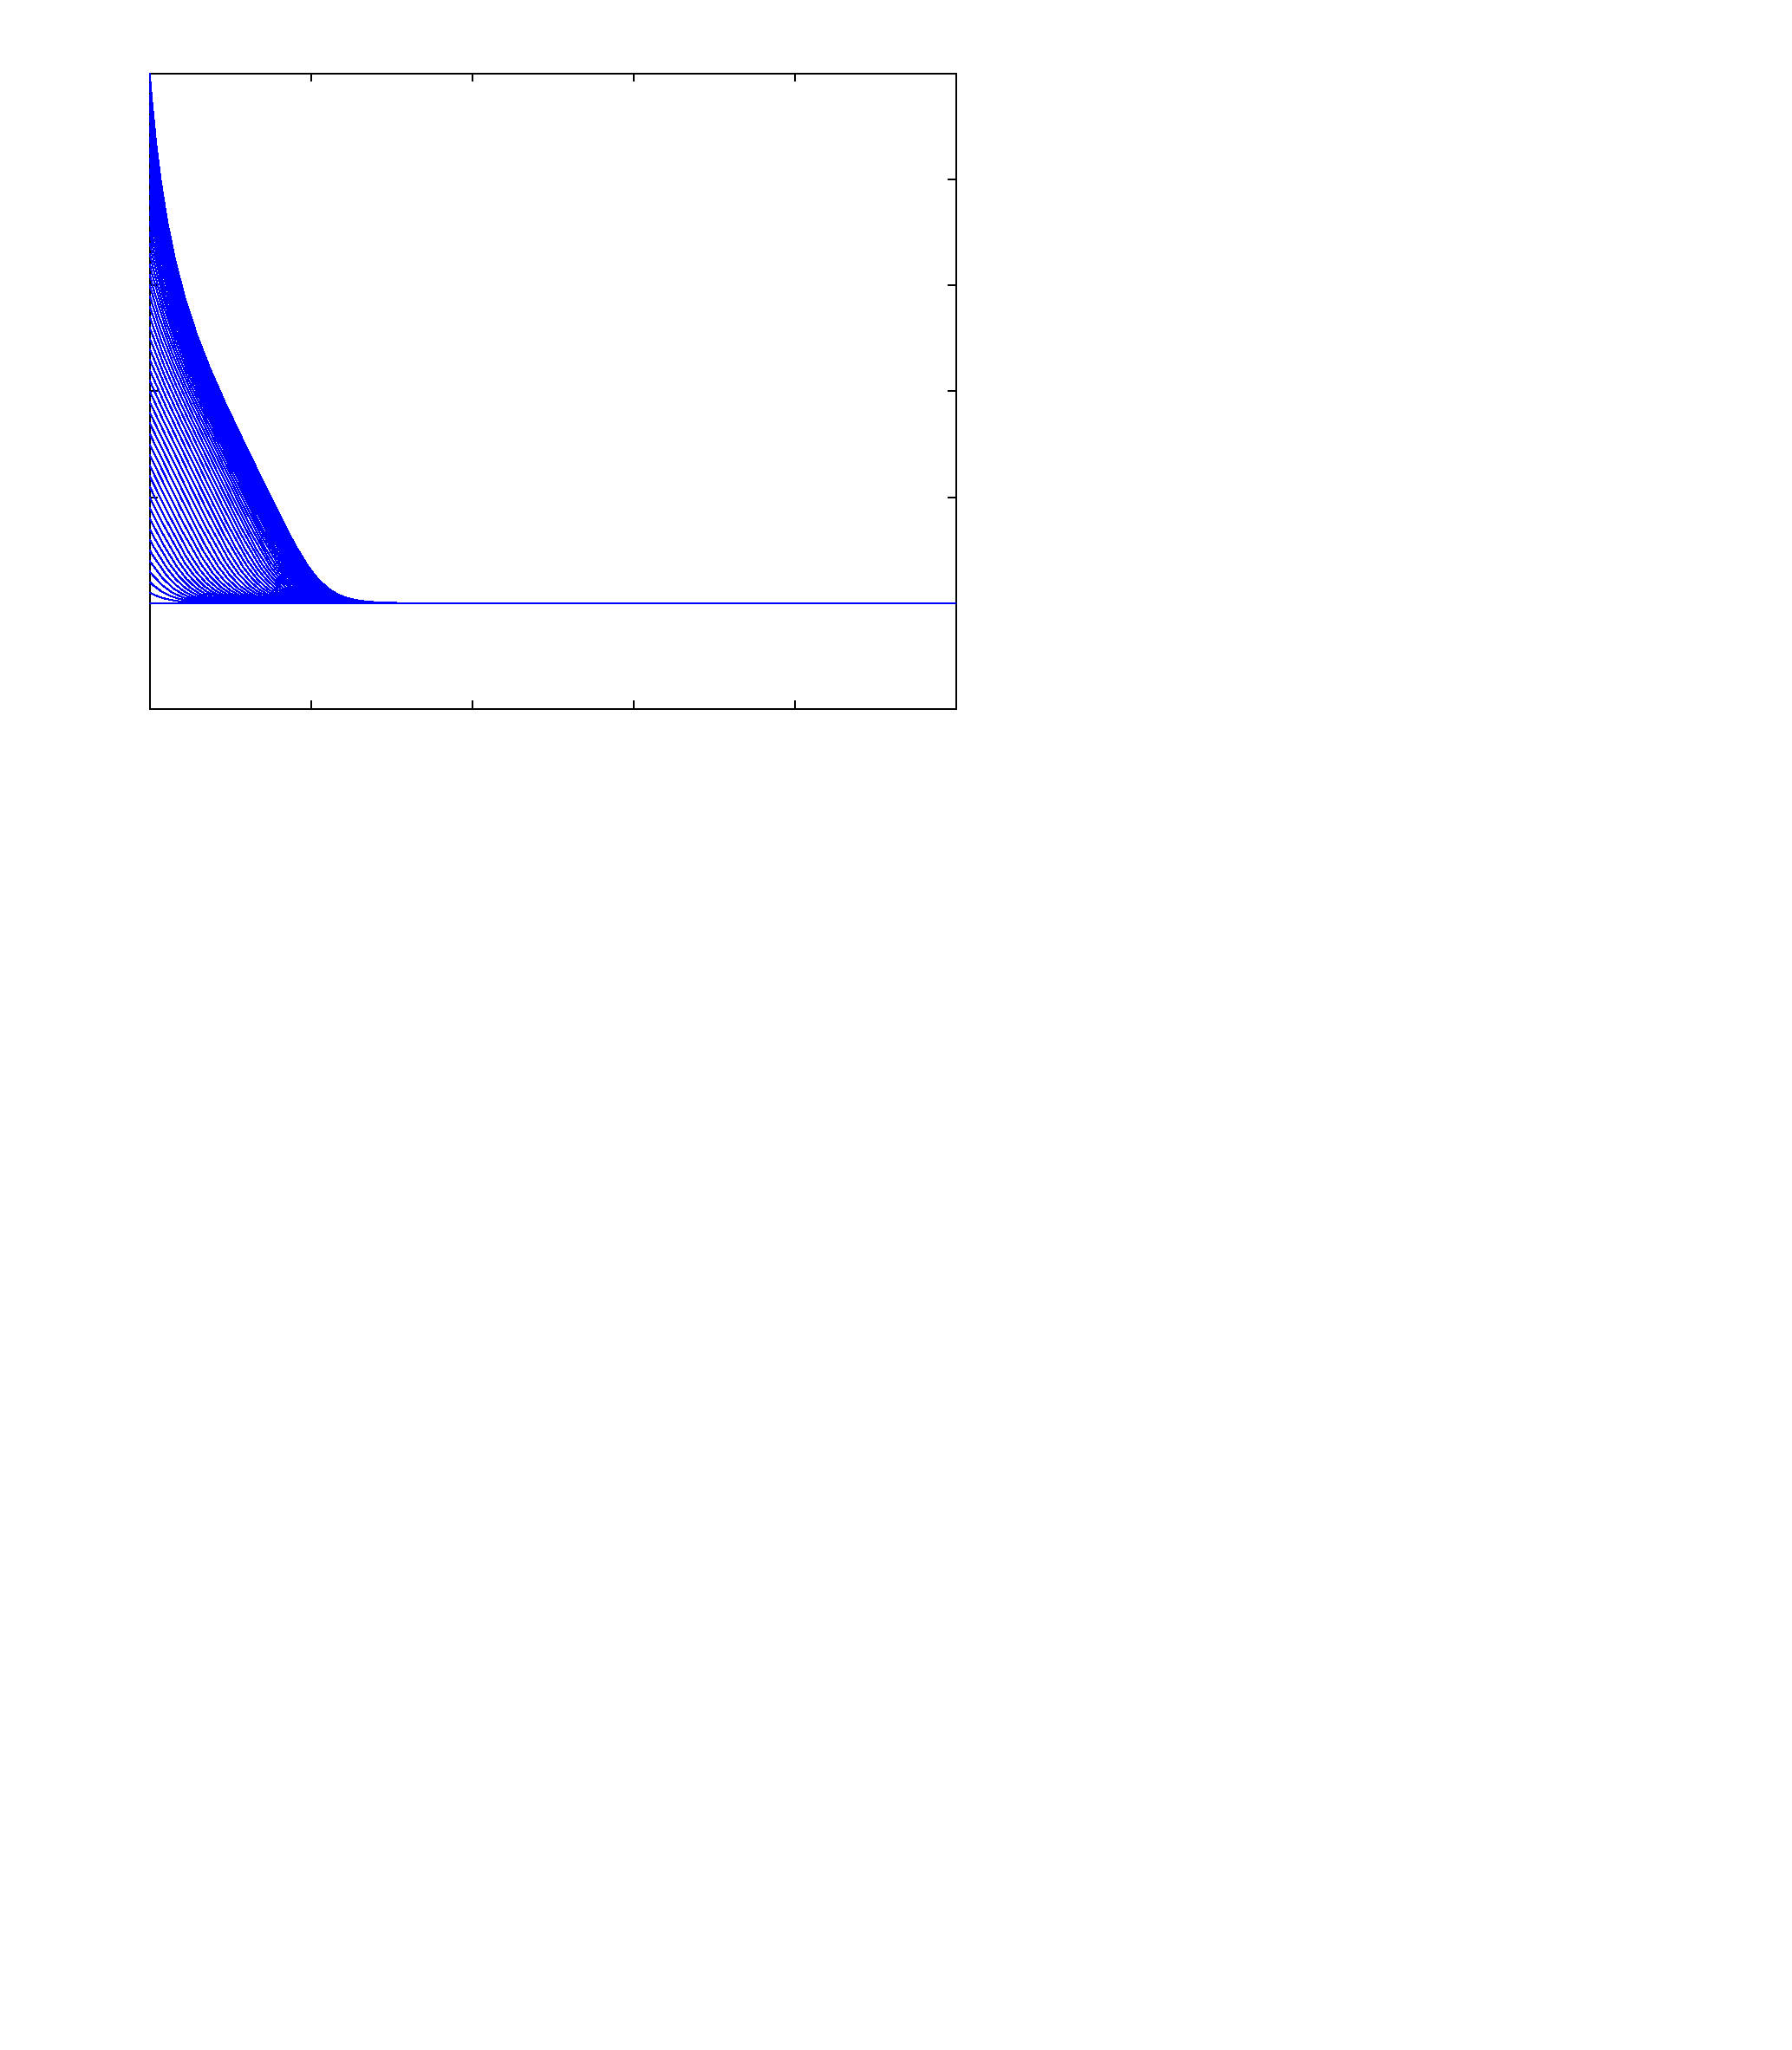
\includegraphics{prog3_fig5-inc}
\end{picture}%
\begin{picture}(976,1119)(0,0)
\fontsize{10}{0}
\selectfont\put(74.88,729.519){\makebox(0,0)[t]{\textcolor[rgb]{0,0,0}{{0}}}}
\fontsize{10}{0}
\selectfont\put(164.16,729.519){\makebox(0,0)[t]{\textcolor[rgb]{0,0,0}{{10}}}}
\fontsize{10}{0}
\selectfont\put(253.44,729.519){\makebox(0,0)[t]{\textcolor[rgb]{0,0,0}{{20}}}}
\fontsize{10}{0}
\selectfont\put(342.72,729.519){\makebox(0,0)[t]{\textcolor[rgb]{0,0,0}{{30}}}}
\fontsize{10}{0}
\selectfont\put(432,729.519){\makebox(0,0)[t]{\textcolor[rgb]{0,0,0}{{40}}}}
\fontsize{10}{0}
\selectfont\put(521.28,729.519){\makebox(0,0)[t]{\textcolor[rgb]{0,0,0}{{50}}}}
\fontsize{10}{0}
\selectfont\put(69.8755,734.52){\makebox(0,0)[r]{\textcolor[rgb]{0,0,0}{{-0.2}}}}
\fontsize{10}{0}
\selectfont\put(69.8755,793.2){\makebox(0,0)[r]{\textcolor[rgb]{0,0,0}{{0}}}}
\fontsize{10}{0}
\selectfont\put(69.8755,851.88){\makebox(0,0)[r]{\textcolor[rgb]{0,0,0}{{0.2}}}}
\fontsize{10}{0}
\selectfont\put(69.8755,910.56){\makebox(0,0)[r]{\textcolor[rgb]{0,0,0}{{0.4}}}}
\fontsize{10}{0}
\selectfont\put(69.8755,969.24){\makebox(0,0)[r]{\textcolor[rgb]{0,0,0}{{0.6}}}}
\fontsize{10}{0}
\selectfont\put(69.8755,1027.92){\makebox(0,0)[r]{\textcolor[rgb]{0,0,0}{{0.8}}}}
\fontsize{10}{0}
\selectfont\put(69.8755,1086.6){\makebox(0,0)[r]{\textcolor[rgb]{0,0,0}{{1}}}}
\fontsize{10}{0}
\selectfont\put(298.08,718.519){\makebox(0,0)[t]{\textcolor[rgb]{0,0,0}{{$\tau$}}}}
\fontsize{10}{0}
\selectfont\put(46.8755,910.56){\rotatebox{90}{\makebox(0,0)[b]{\textcolor[rgb]{0,0,0}{{$u$}}}}}
\fontsize{10}{0}
\selectfont\put(298.08,1096.6){\makebox(0,0)[b]{\textcolor[rgb]{0,0,0}{{Solution curves for different initial conditions, $h=2$}}}}
\end{picture}
}
%   \vspace{-28.5em}
%   \caption{$h=2.0$}
% \end{subfigure}
